\section{Procedure for Paper Submission}

Hand in the draft and final version of your article via Assignments on Brightspace. All draft articles are to be peer reviewed by your fellow students in week 4.5. Instructions on the peer review process are to be found on Brightspace in advance.
The deadline for submitting the final version of your scientific article to your tutor and your Scientific Writing lecturer is in week 4.8.

\section{General Guidelines}

Your Scientific Article should be readable on its own. It should not exceed 4000 words, excluding abstract, reference list, captions and appendices. The article should contain at least the following sections:

\begin{itemize}
    \item  Abstract (max. 250 words)
    \item  Introduction
    \item  Description of the Data (optional, to describe the nature of the data set you have used)
    \item  Method
    \item  Results
    \item  Discussion of the Results (Results and Discussion sections may be combined into a Results and Discussion section, if so desired)
    \item  Conclusions
    \item  Acknowledgments
\end{itemize}

\noindent Appendices can be added if appropriate. Instructions on how to write the sections mentioned above will be given in the Scientific Writing lectures.

\section{Detailed Formatting Instructions}

If you are using this document to prepare your Scientific Article, you can add new files and input them and/or use pre-existing files and type your own text.

\subsection{Document Text}
The default font for your report is Times New Roman, 11-point size. The first line of every paragraph should be indented, with the exception of paragraphs that follow a heading or a blank line (in case of the latter, use \textbackslash noindent). All lines should be single-spaced. Default margins are 1” on all sides. In the electronic version of this template, all margins and other formatting is preset. Limit the use of abbreviations such as e.g. or viz.

\subsection{Headings}
The title of your paper should be typed in bold, 18-point type, with capital and lower-case letters, and centered at the top of the page. The names of the authors and the affiliation should follow on separate lines below the title. Author names are centered, and affiliations are centered and in italic type.

\begin{itemize}
    \item Major headings (\textbackslash sections\{\}) are bold 11-point font, centered, and numbered with Roman numerals.
    \item Subheadings (\textbackslash subsections\{\}) are bold, flush left, and numbered with capital letters.
    \item Sub-subheadings (\textbackslash subsubsections\{\}) are italic, flush left, and numbered (1. 2. 3. etc.)
\end{itemize}

\subsection{In-text References}
Choose and output style that you will use for your references and apply this style consistently throughout your paper. Make sure that you know what your in text references should look like and how different publication types (e.g. books, journal papers etc.) should  be formatted in the reference list.  Examples of references styles are: 

\begin{itemize}
    \item IAA, in which the references are numbered following the order of appearance in your text (for examples of titles in the Reference list, see the “References” section on page 4 of this template. For documentation, see sample.bib), and
    \item APA, in which you present the name(s) of the author(s) and the year of publication in your text and references are sorted alphabetically in the reference list.  	
\end{itemize}

\subsection{Footnotes}
Footnotes, where they appear, should be placed above the 1” margin at the bottom of the page. To insert footnotes into the template, use \textbackslash footnote\{\}. Use superscript numbers for footnotes (which is by default already the case). Use footnotes scarcely and only to provide additional information that is not essential to understand your argumentation in the main text. 

\subsection{Images, Figures, and Tables}
Captions are bold and justified, with a period and a single tab (no hyphen or other character) between the figure number and figure description.

Place figure captions below all figures; place table titles over the tables. If your figure has multiple parts, include the labels “a),” “b),” etc. below and to the left of each part, above the figure caption. Please verify that the figures and tables you mention in the text actually exist. When citing a figure in the text, use the abbreviation “Fig.” except at the beginning of a sentence. Do not abbreviate “Table.” Number each different type of illustration (i.e., figures, tables) sequentially with relation to other illustrations of the same type.

Figure axis labels are often a source of confusion. Use words rather than symbols. As in the example below (\autoref{fig:sample}), write the quantity “Magnetization” rather than just “M.” Do not label axes with units only. 
Figure labels must be legible, approximately 8-12 point type. Only use colors for your illustrations if needed. 

\begin{figure}[h]
    \centering
    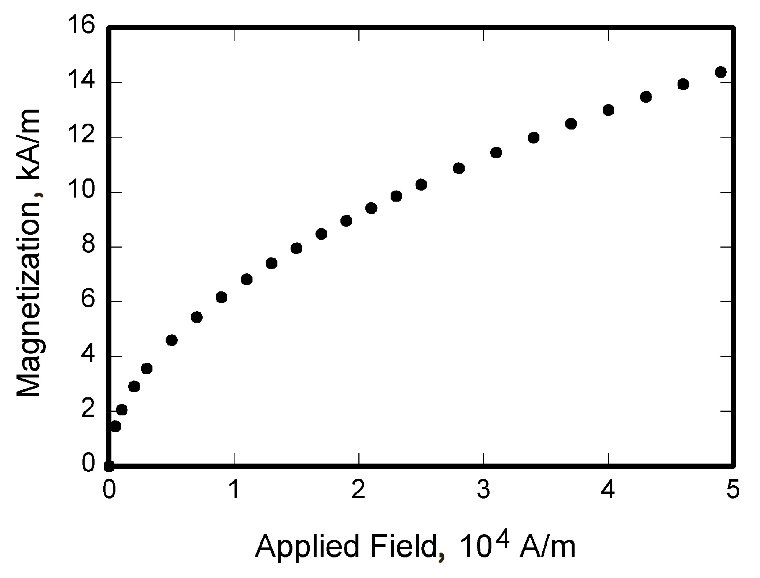
\includegraphics[width=0.4\linewidth]{figures/graph.jpg}
    \caption{Magnetization as a function of applied field}
    \label{fig:sample}
\end{figure}

\subsection{Equations, Numbers, Symbols, and Abbreviations}
Equations are centered and numbered consecutively, with equation numbers in parentheses flush right, as in \ref{eqn:sample}. Insert a blank line on either side of the equation.
\begin{equation}
    \label{eqn:sample}
    L = C_L \frac{1}{2}\rho V^2 S
\end{equation}

\noindent Be sure that the symbols in your equation are defined before the equation appears, or immediately following. Italicize symbols (T might refer to temperature, but T is the unit tesla). Refer to “Eq. (1),” not “(1)” or “equation (1)” except at the beginning of a sentence: “Equation (1) is…”

Define abbreviations and acronyms the first time they are used in the text, even after they have already been defined in the abstract. Do not use abbreviations in the title.
